%\documentclass[10pt]{beamer} % aspect ratio 4:3, 128 mm by 96 mm
\documentclass[10pt,aspectratio=169]{beamer} % aspect ratio 16:9
%\graphicspath{{../../figures/}}
\graphicspath{{../../figures/}{../../figures/beamer_common/}{../../conference_papers/SPIE2020/figs/}{../../journal_papers/Composite_Structures_GA/figs/}}
%\includeonlyframes{frame1,frame2,frame3,frame4,frame5,frame6,frame7,frame8,frame9}
%\includeonlyframes{frame10,frame11,frame12,frame13}
%\includeonlyframes{frame14,frame15,frame16,frame17,frame18,frame19,frame20,frame21}
%\includeonlyframes{frame22,frame23,frame24,frame25,frame26}
%\includeonlyframes{frame27,frame28}
%%%%%%%%%%%%%%%%%%%%%%%%%%%%%%%%%%%%%%%%%%%%%%%%%%
% Packages
%%%%%%%%%%%%%%%%%%%%%%%%%%%%%%%%%%%%%%%%%%%%%%%%%%
\usepackage{appendixnumberbeamer}
\usepackage{booktabs}
\usepackage{csvsimple} % for csv read
\usepackage[scale=2]{ccicons}
\usepackage{pgfplots}
\usepackage{xspace}
\usepackage{amsmath}
\usepackage{totcount}
\usepackage{tikz}
\usepackage{bm}
%\usepackage{FiraSans}

%\usepackage{comment}
%\usetikzlibrary{external} % speedup compilation
%\tikzexternalize % activate!
%\usetikzlibrary{shapes,arrows}  

%\usepackage{bibentry}
%\nobibliography*
\usepackage{caption}%
\captionsetup[figure]{labelformat=empty}%
%%%%%%%%%%%%%%%%%%%%%%%%%%%%%%%%%%%%%%%%%%%%%%%%%%
% Metropolis theme custom modification file
%%%%%%%%%%%%%%%%%%%%%%%%%%%%%%%%%%%%%%%%%%%%%%%%%%
% Metropolis theme custom modification file
%%%%%%%%%%%%%%%%%%%%%%%%%%%%%%%%%%%%%%%%%%%%%%%%%%
% Metropolis theme custom colors
%%%%%%%%%%%%%%%%%%%%%%%%%%%%%%%%%%%%%%%%%%%%%%%%%%
\usetheme[progressbar=foot]{metropolis}
\useoutertheme{metropolis}
\useinnertheme{metropolis}
\usefonttheme{metropolis}
\setbeamercolor{background canvas}{bg=white}

%\usecolortheme{spruce}

\definecolor{myblue}{rgb}{0.19,0.55,0.91}
\definecolor{mediumblue}{rgb}{0,0,205}
\definecolor{darkblue}{rgb}{0,0,139}
\definecolor{Dodgerblue}{HTML}{1E90FF}
\definecolor{Navy}{HTML}{000080} % {rgb}{0,0,128}
\definecolor{Aliceblue}{HTML}{F0F8FF}
\definecolor{Lightskyblue}{HTML}{87CEFA}
\definecolor{logoblue}{RGB}{1,67,140}
\definecolor{Purple}{HTML}{911146}
\definecolor{Orange}{HTML}{CF4A30}

\setbeamercolor{progress bar}{bg=Lightskyblue}
\setbeamercolor{progress bar}{ fg=logoblue} 
\setbeamercolor{frametitle}{bg=logoblue}
\setbeamercolor{title separator}{fg=logoblue}
\setbeamercolor{block title}{bg=Lightskyblue!30,fg=black}
\setbeamercolor{block body}{bg=Lightskyblue!15,fg=black}
\setbeamercolor{alerted text}{fg=Purple}
%%%%%%%%%%%%%%%%%%%%%%%%%%%%%%%%%%%%%%%%%%%%%%%%%%
%  Theme modifications
%%%%%%%%%%%%%%%%%%%%%%%%%%%%%%%%%%%%%%%%%%%%%%%%%%
% modify progress bar linewidth
\makeatletter
\setlength{\metropolis@progressinheadfoot@linewidth}{2pt} 
\setlength{\metropolis@titleseparator@linewidth}{1pt}
\setlength{\metropolis@progressonsectionpage@linewidth}{1pt}

\setbeamertemplate{progress bar in section page}{
	\setlength{\metropolis@progressonsectionpage}{%
		\textwidth * \ratio{\thesection pt}{\totvalue{totalsection} pt}%
	}%
	\begin{tikzpicture}
	\fill[bg] (0,0) rectangle (\textwidth, \metropolis@progressonsectionpage@linewidth);
	\fill[fg] (0,0) rectangle (\metropolis@progressonsectionpage, \metropolis@progressonsectionpage@linewidth);
	\end{tikzpicture}%
}
\makeatother
\newcounter{totalsection}
\regtotcounter{totalsection}

\AtBeginDocument{%
	\pretocmd{\section}{\refstepcounter{totalsection}}{\typeout{Yes, prepending was successful}}{\typeout{No, prepending was not successful}}%
}%
%%%%%%%%%%%%%%%%%%%%%%%%%%%%%%%%%%%%%%%%%%%%%%%%%%
%  Bibliography mods
%%%%%%%%%%%%%%%%%%%%%%%%%%%%%%%%%%%%%%%%%%%%%%%%%%
\setbeamertemplate{bibliography item}{\insertbiblabel} %% Remove book symbol from references and add number in square brackets
% kill the abominable icon (without number)
%\setbeamertemplate{bibliography item}{}
%\makeatletter
%\renewcommand\@biblabel[1]{#1.} % number only
%\makeatother
% remove line breaks in bibliography
\setbeamertemplate{bibliography entry title}{}
\setbeamertemplate{bibliography entry location}{}
%%%%%%%%%%%%%%%%%%%%%%%%%%%%%%%%%%%%%%%%%%%%%%%%%%
%  Bibliography custom commands
%%%%%%%%%%%%%%%%%%%%%%%%%%%%%%%%%%%%%%%%%%%%%%%%%%
\newcommand{\bibliotitlestyle}[1]{\textbf{#1}\par}

\newif\ifinbiblio
\newcounter{bibkey}
\newenvironment{biblio}[2][long]{%
    %\setbeamertemplate{bibliography item}{\insertbiblabel}
    \setbeamertemplate{bibliography item}{}% without numbers
	\setbeamerfont{bibliography item}{size=\footnotesize}
	\setbeamerfont{bibliography entry author}{size=\footnotesize}
	\setbeamerfont{bibliography entry title}{size=\footnotesize}
	\setbeamerfont{bibliography entry location}{size=\footnotesize}
	\setbeamerfont{bibliography entry note}{size=\footnotesize}
	\ifx!#2!\else%
	\bibliotitlestyle{#2}%
	\fi%
	\begin{thebibliography}{}%
		\inbibliotrue%
		\setbeamertemplate{bibliography entry title}[#1]%
	}{%
		\inbibliofalse%
		\setbeamertemplate{bibliography item}{}%
	\end{thebibliography}%
}

\newcommand{\biblioref}[5][short]{
	\setbeamertemplate{bibliography entry title}[#1]
	\stepcounter{bibkey}%
	\ifinbiblio%
	\bibitem{\thebibkey}%
	#2
	\newblock #4
	\ifx!#5!\else\newblock {\em #5}, #3 \fi%
	\else%
	\begin{biblio}{}
		\bibitem{\thebibkey}
		#2
		\newblock #4
		\ifx!#5!\else\newblock {\em #5}, #3\fi
	\end{biblio}
	\fi
}
%
%\newbibmacro*{hypercite}{%
%	\renewcommand{\@makefntext}[1]{\noindent\normalfont##1}%
%	\footnotetext{%
%		\blxmkbibnote{foot}{%
%			\printtext[labelnumberwidth]{%
%				\printfield{prefixnumber}%
%				\printfield{labelnumber}}%
%			\addspace
%			\fullcite{\thefield{entrykey}}}}}
%
%\DeclareCiteCommand{\hypercite}%
%{\usebibmacro{cite:init}}
%{\usebibmacro{hypercite}}
%{}
%{\usebibmacro{cite:dump}}
%
%% Redefine the \footfullcite command to use the reference number
%\renewcommand{\footfullcite}[1]{\cite{#1}\hypercite{#1}}
\usefonttheme[onlymath]{Serif} 

%%%%%%%%%%%%%%%%%%%%%%%%%%%%%%%%%%%%%%%%%%%%%%%%%%
% Custom commands
%%%%%%%%%%%%%%%%%%%%%%%%%%%%%%%%%%%%%%%%%%%%%%%%%%
% matrix command 
\newcommand{\matr}[1]{\mathbf{#1}} % bold upright (Elsevier, Springer)
%\newcommand{\matr}[1]{#1}          % pure math version
%\newcommand{\matr}[1]{\bm{#1}}     % ISO complying version
% vector command 
\newcommand{\vect}[1]{\mathbf{#1}} % bold upright (Elsevier, Springer)
% bold symbol
\newcommand{\bs}[1]{\boldsymbol{#1}}
% derivative upright command
\DeclareRobustCommand*{\drv}{\mathop{}\!\mathrm{d}}
\newcommand{\ud}{\mathrm{d}}
% 
\newcommand{\themename}{\textbf{\textsc{metropolis}}\xspace}

%%%%%%%%%%%%%%%%%%%%%%%%%%%%%%%%%%%%%%%%%%%%%%%%%%
%  Title page options
%%%%%%%%%%%%%%%%%%%%%%%%%%%%%%%%%%%%%%%%%%%%%%%%%%
% \date{\today}
\date{}
%%%%%%%%%%%%%%%%%%%%%%%%%%%%%%%%%%%%%%%%%%%%%%%%%%
% option 1
%%%%%%%%%%%%%%%%%%%%%%%%%%%%%%%%%%%%%%%%%%%%%%%%%%
\title{Parametric studies of composite material properties influence on dispersion curves of Lamb waves}
\subtitle{Lamb-opt}
\author{\textbf{Paweł Kudela}\\Piotr Fiborek\\Maciej Radzieński \\Tomasz Wandowski }
% logo align to Institute 
\institute{Institute of Fluid Flow Machinery\\Polish Academy of Sciences \\ \vspace{-1.5cm}\flushright 
\includegraphics[width=4cm]{../images/logo/logo_eng_40mm.eps}}
%%%%%%%%%%%%%%%%%%%%%%%%%%%%%%%%%%%%%%%%%%%%%%%%%%
% option 2 - authors in one line
%%%%%%%%%%%%%%%%%%%%%%%%%%%%%%%%%%%%%%%%%%%%%%%%%%
%	\title{Elastic constants identification of composite laminates by using Lamb wave dispersion curves and optimization methods}
%	\subtitle{Lamb-opt}
%	\author{\textbf{Paweł Kudela}\textsuperscript{2}, Maciej Radzieński\textsuperscript{2}, Wiesław Ostachowicz\textsuperscript{2}, Zhibo Yang\textsuperscript{1} }
%	% logo align to Institute 
%	\institute{\textsuperscript{1}Xi'an Jiaotong University \\ \textsuperscript{2}Institute of Fluid Flow Machinery\\ \hspace*{1pt} Polish Academy of Sciences \\ \vspace{-1.5cm}\flushright 
\includegraphics[width=4cm]{../images/logo/logo_eng_40mm.eps}}
%%%%%%%%%%%%%%%%%%%%%%%%%%%%%%%%%%%%%%%%%%%%%%%%%%
% option 3 - multilogo vertical
%%%%%%%%%%%%%%%%%%%%%%%%%%%%%%%%%%%%%%%%%%%%%%%%%%
%\title{Elastic constants identification of composite laminates by using Lamb wave dispersion curves and optimization methods}
%\subtitle{Lamb-opt}
%	\author{\textbf{Paweł Kudela}\inst{1}, Maciej Radzieński\inst{1}, Wiesław Ostachowicz\inst{1}, Zhibo Yang\inst{2} }
%	% logo under Institute 
%	\institute%
%	{ 
%		\inst{1}%
%		Institute of Fluid Flow Machinery\\ \hspace*{1pt} Polish Academy of Sciences \\ 
\includegraphics[height=0.85cm]{../images/logo/logo_eng_40mm.eps} \\
%		\and
%		\inst{2}%
%	    Xi'an Jiaotong University \\ 
\includegraphics[height=0.85cm]{../images/logo/logo_box.eps}
%    }
% end od option 3
%%%%%%%%%%%%%%%%%%%%%%%%%%%%%%%%%%%%%%%%%%%%%%%%%%
%% option 4 - 3 Institutes and logos horizontal centered
%%%%%%%%%%%%%%%%%%%%%%%%%%%%%%%%%%%%%%%%%%%%%%%%%%
%\title{Elastic constants identification of composite laminates by using Lamb wave dispersion curves and optimization methods}
%\subtitle{Lamb-opt }
%\author{\textbf{Paweł Kudela}\textsuperscript{1}, Maciej Radzieński\textsuperscript{1}, Marco Miniaci\textsuperscript{2}, Zhibo Yang\textsuperscript{3} }
%
%\institute{ 
%\begin{columns}[T,onlytextwidth]
%	\column{0.39\textwidth}
%	\begin{center}
%		\textsuperscript{1}Institute of Fluid Flow Machinery\\ \hspace*{3pt}Polish Academy of Sciences
%	\end{center}
%	\column{0.3\textwidth}
%	\begin{center}
%		\textsuperscript{2}Zurich University
%	\end{center}
%	\column{0.3\textwidth}
%	\begin{center}
%		\textsuperscript{3}Xi'an Jiaotong University
%	\end{center}
%\end{columns}
%\vspace{6pt}
%% logos 
%\begin{columns}[b,onlytextwidth]
%	\column{0.39\textwidth}
%		\centering 
%		
\includegraphics[scale=0.9,height=0.85cm,keepaspectratio]{../images/logo/logo_eng_40mm.eps}
%	\column{0.3\textwidth}
%		\centering 
%		
\includegraphics[scale=0.9,height=0.85cm,keepaspectratio]{../images/logo/logo_box.eps}
%	\column{0.3\textwidth}
%		\centering 
%		
\includegraphics[scale=0.9,height=0.85cm,keepaspectratio]{../images/logo/logo_box2.eps}
%\end{columns}
%}
%\makeatletter
%\setbeamertemplate{title page}{
%	\begin{minipage}[b][\paperheight]{\textwidth}
%		\centering  % <-- Center here
%		\ifx\inserttitlegraphic\@empty\else\usebeamertemplate*{title graphic}\fi
%		\vfill%
%		\ifx\inserttitle\@empty\else\usebeamertemplate*{title}\fi
%		\ifx\insertsubtitle\@empty\else\usebeamertemplate*{subtitle}\fi
%		\usebeamertemplate*{title separator}
%		\ifx\beamer@shortauthor\@empty\else\usebeamertemplate*{author}\fi
%		\ifx\insertdate\@empty\else\usebeamertemplate*{date}\fi
%		\ifx\insertinstitute\@empty\else\usebeamertemplate*{institute}\fi
%		\vfill
%		\vspace*{1mm}
%	\end{minipage}
%}
%
%\setbeamertemplate{title}{
%	%  \raggedright%  % <-- Comment here
%	\linespread{1.0}%
%	\inserttitle%
%	\par%
%	\vspace*{0.5em}
%}
%\setbeamertemplate{subtitle}{
%	%  \raggedright%  % <-- Comment here
%	\insertsubtitle%
%	\par%
%	\vspace*{0.5em}
%}
%\makeatother
% end of option 4
%%%%%%%%%%%%%%%%%%%%%%%%%%%%%%%%%%%%%%%%%%%%%%%%%%
% option 5 - 2 Institutes and logos horizontal centered
%%%%%%%%%%%%%%%%%%%%%%%%%%%%%%%%%%%%%%%%%%%%%%%%%%
%\title{Elastic constants identification of composite laminates by using Lamb wave dispersion curves and optimization methods}
%\subtitle{Lamb-opt }
%\author{\textbf{Paweł Kudela}\textsuperscript{1}, Maciej Radzieński\textsuperscript{1}, Marco Miniaci\textsuperscript{2}}
%
%\institute{ 
%	\begin{columns}[T,onlytextwidth]
%		\column{0.5\textwidth}
%			\centering
%			\textsuperscript{1}Institute of Fluid Flow Machinery\\ \hspace*{3pt}Polish Academy of Sciences
%		\column{0.5\textwidth}
%			\centering
%			\textsuperscript{2}Zurich University
%	\end{columns}
%	\vspace{6pt}
%	% logos 
%	\begin{columns}[b,onlytextwidth]
%		\column{0.5\textwidth}
%		\centering 
%		
\includegraphics[scale=0.9,height=0.85cm,keepaspectratio]{../images/logo/logo_eng_40mm.eps}
%		\column{0.5\textwidth}
%		\centering 
%		
\includegraphics[scale=0.9,height=0.85cm,keepaspectratio]{../images/logo/logo_box.eps}
%	\end{columns}
%}
%\makeatletter
%\setbeamertemplate{title page}{
%	\begin{minipage}[b][\paperheight]{\textwidth}
%		\centering  % <-- Center here
%		\ifx\inserttitlegraphic\@empty\else\usebeamertemplate*{title graphic}\fi
%		\vfill%
%		\ifx\inserttitle\@empty\else\usebeamertemplate*{title}\fi
%		\ifx\insertsubtitle\@empty\else\usebeamertemplate*{subtitle}\fi
%		\usebeamertemplate*{title separator}
%		\ifx\beamer@shortauthor\@empty\else\usebeamertemplate*{author}\fi
%		\ifx\insertdate\@empty\else\usebeamertemplate*{date}\fi
%		\ifx\insertinstitute\@empty\else\usebeamertemplate*{institute}\fi
%		\vfill
%		\vspace*{1mm}
%	\end{minipage}
%}
%
%\setbeamertemplate{title}{
%	%  \raggedright%  % <-- Comment here
%	\linespread{1.0}%
%	\inserttitle%
%	\par%
%	\vspace*{0.5em}
%}
%\setbeamertemplate{subtitle}{
%	%  \raggedright%  % <-- Comment here
%	\insertsubtitle%
%	\par%
%	\vspace*{0.5em}
%}
%\makeatother
% end of option 5
%
%%%%%%%%%%%%%%%%%%%%%%%%%%%%%%%%%%%%%%%%%%%%%%%%%%
%  End of title page options
%%%%%%%%%%%%%%%%%%%%%%%%%%%%%%%%%%%%%%%%%%%%%%%%%%
% logo option - alternative manual insertion by modification of coordinates in \put()
%\titlegraphic{%
%	%\vspace{\logoadheight}
%	\begin{picture}(0,0)
%	\put(305,-185){\makebox(0,0)[rb]{
\includegraphics[width=4cm]{../images/logo/logo_eng_40mm.eps}}}
%	\end{picture}}
%
%%%%%%%%%%%%%%%%%%%%%%%%%%%%%%%%%%%%%%%%%%%%%%%%%%
%\tikzexternalize % activate!
%%%%%%%%%%%%%%%%%%%%%%%%%%%%%%%%%%%%%%%%%%%%%%%%%%
\begin{document}
%%%%%%%%%%%%%%%%%%%%%%%%%%%%%%%%%%%%%%%%%%%%%%%%%%
\maketitle
%%%%%%%%%%%%%%%%%%%%%%%%%%%%%%%%%%%%%%%%%%%%%%%%%%
% SLIDES
%%%%%%%%%%%%%%%%%%%%%%%%%%%%%%%%%%%%%%%%%%%%%%%%%%
\begin{frame}[label=frame1]{Table of contents \label{frameone}}
  \setbeamertemplate{section in toc}[sections numbered]
  \tableofcontents[hideallsubsections]
\end{frame}
%%%%%%%%%%%%%%%%%%%%%%%%%%%%%%%%%%%%%%%%%%%%%%%%%%
\section{Introduction}
%%%%%%%%%%%%%%%%%%%%%%%%%%%%%%%%%%%%%%%%%%%%%%%%%%

%%%%%%%%%%%%%%%%%%%%%%%%%%%%%%%%%%%%%%%%%%%%%%%%%%
\begin{frame}[label=frame2]{Determination of mechanical properties of materials}
  \begin{itemize}
  	\item Destructive testing
  	\item Static tests (displacement measurements + model)
  	\item Dynamic tests (natural frequencies)
  	\item Ultrasonic methods (bulk wave velocities, ultrasonic polar scan)
  	\item \textbf{Lamb wave methods (dispersion curves)}
  \end{itemize}
\end{frame}
%%%%%%%%%%%%%%%%%%%%%%%%%%%%%%%%%%%%%%%%%%%%%%%%%%

%%%%%%%%%%%%%%%%%%%%%%%%%%%%%%%%%%%%%%%%%%%%%%%%%%
\begin{frame}[label=frame3]{Idea of the project}
\begin{figure}
	\only<1>{
		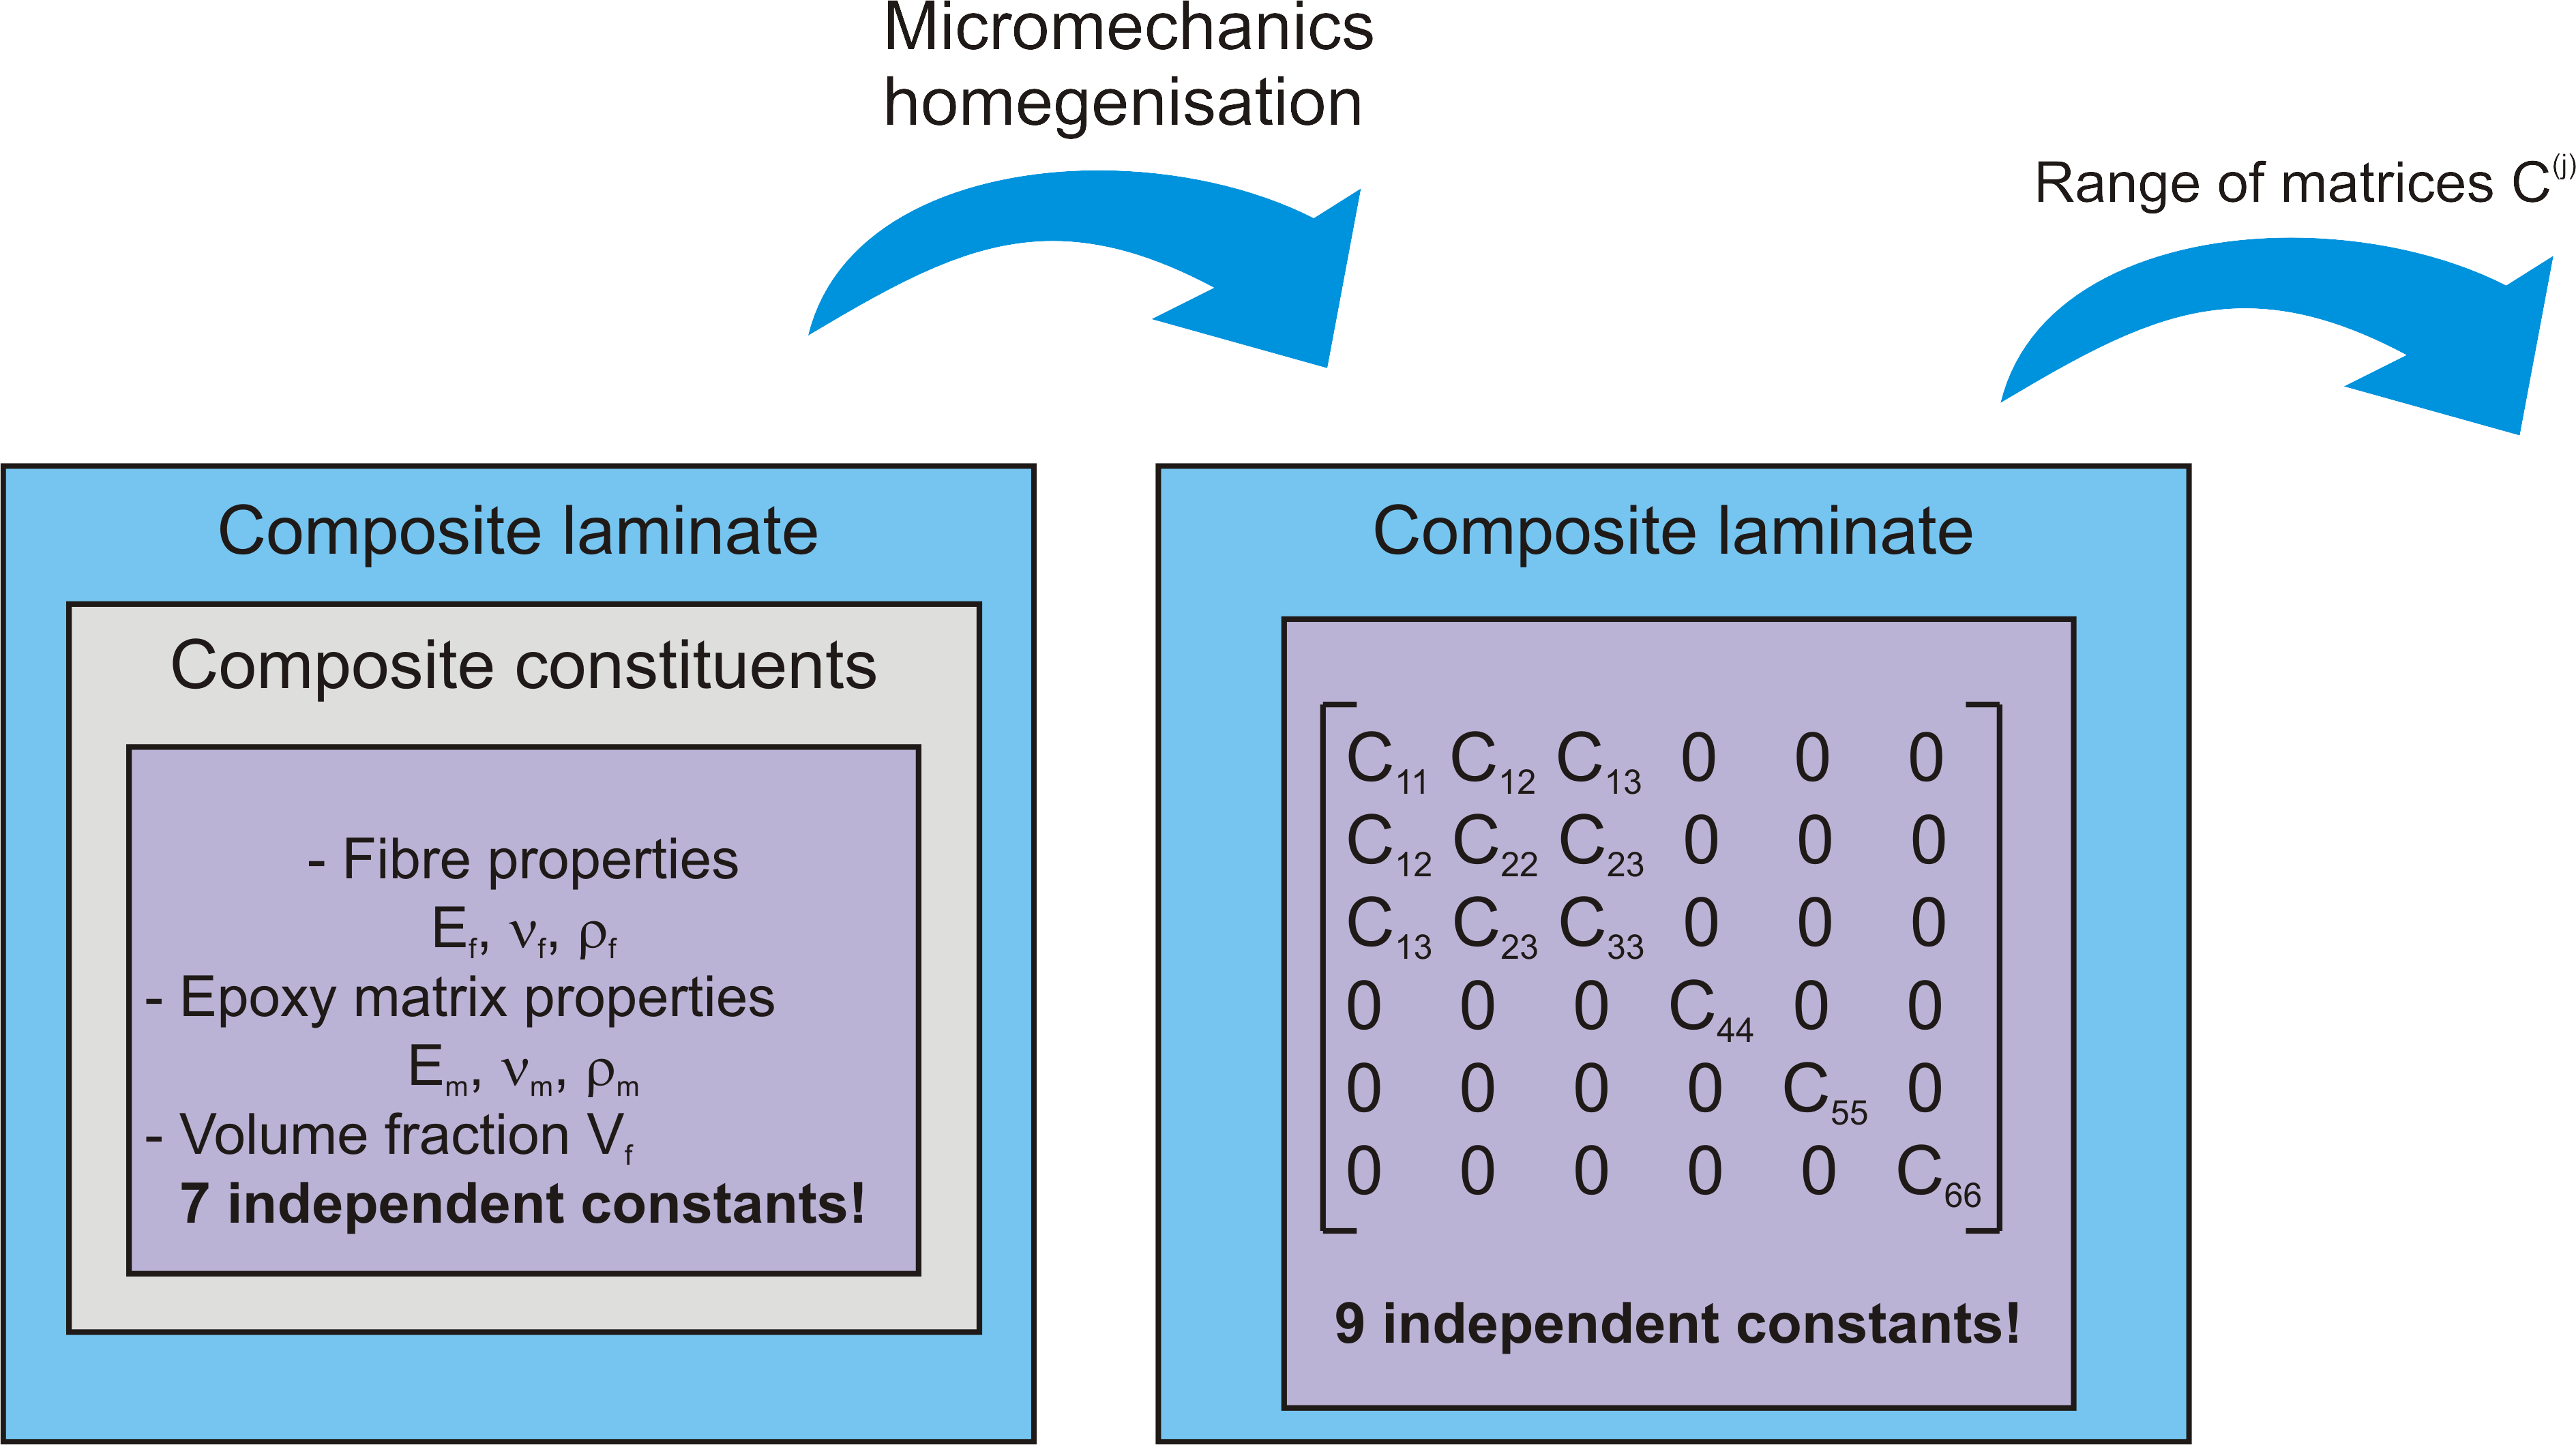
\includegraphics[width=0.8\textwidth]{Plan-scheme4a.png}
	}
	\only<2>{
		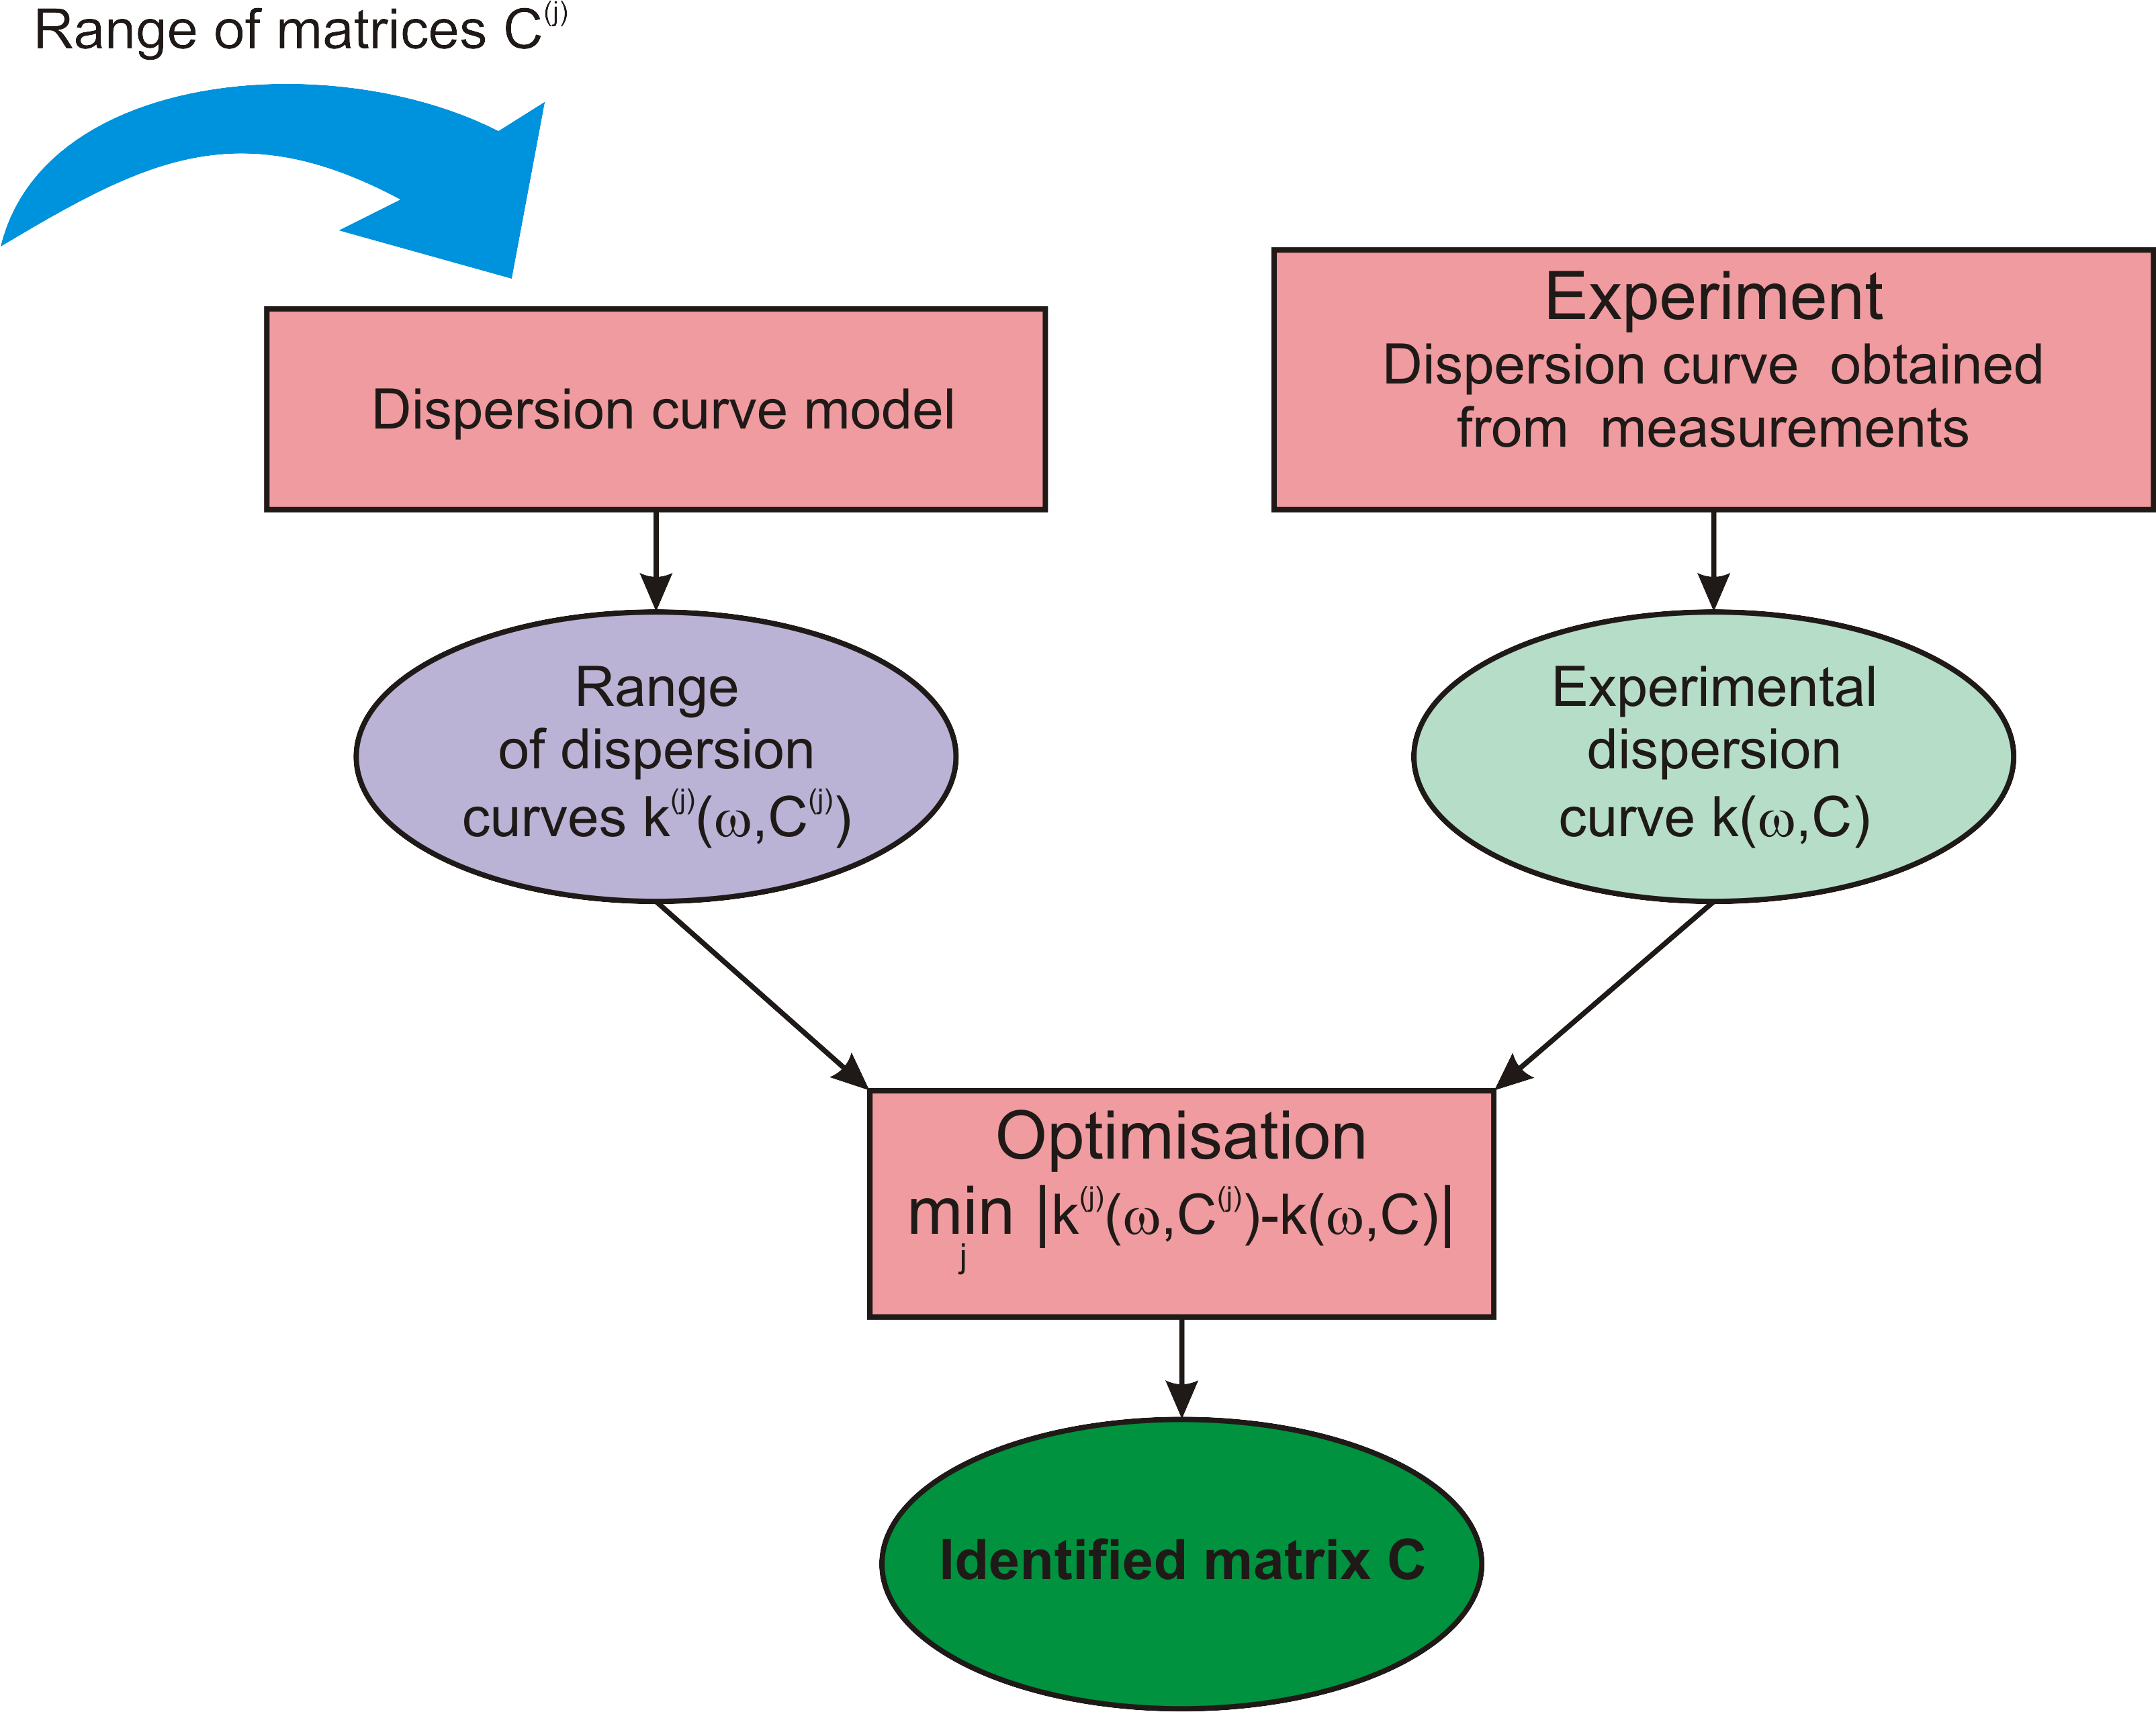
\includegraphics[width=0.65\textwidth]{Plan-scheme4b.png}
	}
\end{figure}
\only<1>{
		\begin{columns}[T]
		\column{0.5\textwidth}
		\hspace{1.5cm} \(E_f=E_{11f}\) \quad \(E_{22f}=0.1 E_{11f}\)
			\column{0.5\textwidth}
		\(\bs{\sigma} = \matr{C} \, \bs{\varepsilon}\)
	\end{columns}
}
\end{frame}
%%%%%%%%%%%%%%%%%%%%%%%%%%%%%%%%%%%%%%%%%%%%%%%%%%
%%%%%%%%%%%%%%%%%%%%%%%%%%%%%%%%%%%%%%%%%%%%%%%%%%
\begin{frame}[label=frame4]{Dispersion curves (1)}
	\begin{alertblock}{Definition}
		A \textbf{dispersion relation} relates the wavelength $\lambda$ or wavenumber $k$ of a wave to its frequency $\omega$.\\
		 \vspace{10pt}
		$k(\omega)$ $[\frac{\mathrm{rad}}{\mathrm{m}}]$\\
			 \vspace{6pt}
		$k(f)$ $[\frac{1}{\mathrm{m}}]$
	\end{alertblock}
	\begin{block}{Phase velocity}
		\begin{equation*}
			c_p = \frac{\omega}{k}
		\end{equation*}
	\end{block}
\begin{block}{Group velocity}
	\begin{equation*}
	c_g = \frac{\drv \omega}{\drv k}
	\end{equation*}
\end{block}
\end{frame}
%%%%%%%%%%%%%%%%%%%%%%%%%%%%%%%%%%%%%%%%%%%%%%%%%%
\section{Semi Analytical Spectral Element Method (SASE)}
%%%%%%%%%%%%%%%%%%%%%%%%%%%%%%%%%%%%%%%%%%%%%%%%%%
\begin{frame}[label=frame9]{Semi Analytical Spectral Element Method (SASE)}
	\begin{figure}
		\includegraphics[width=\textwidth]{figure1.png}
	\end{figure}
	\begin{equation*}
	\vect{u}(x,y,z,t) = \matr{U}(x) \exp \left[ i (\omega t + k \sin (\beta) y - k \cos (\beta) z)\right]
	\end{equation*}
\end{frame}
%%%%%%%%%%%%%
\begin{frame}[t,label=frame10]{Semi Analytical Spectral Element Method (SASE)}
\only<1-3>{
	\begin{equation*}
		\left[\matr{A} - \omega^2\matr{M} \right] \vect{U} =0,
		\label{eq:eig_dispersion}
	\end{equation*}
where $\omega$ is the angular frequency, $\matr{M}$ is the mass matrix, $\matr{U}$ is the nodal displacement vector, and the matrix $\matr{A}$ can be defined as:
	\begin{equation*}
		\begin{aligned}
		\matr{A} & =  k^2\left(s^2 \,\matr{K}_{22} + c^2\, \matr{K}_{33} - c s\, \matr{K}_{23} - c s\, \matr{K}_{32}\right) \\
		& + i k\, \matr{T}^T\left(-c\, \matr{K}_{13} - s\, \matr{K}_{21} + s\, \matr{K}_{12} + c\, \matr{K}_{31}\right) \matr{T} +\matr{K}_{11},
		\end{aligned}
		\label{eq:dispersion}
	\end{equation*}
	where  $s = \sin(\beta)$, $c = \cos(\beta)$, $i = \sqrt{-1}$.
}
\only<2-3>{
	\begin{equation*}
		\matr{K}_{mn}^e= \int \limits_{(e)} \matr{B}_m^{T} \matr{C}^e \, \matr{B}_n\, \ud x
		\label{eq:stiffness_matrix_e}
	\end{equation*}
}
\only<3>{
	Possible solutions:
	\begin{columns}[T]
		\column{0.5\textwidth}
		\begin{itemize}
			\item standard eigenvalue problem $\omega (k)$
		\end{itemize}
		\column{0.5\textwidth}
		\begin{itemize}
		\item second-order polynomial eigenvalue problem $k(\omega)$
		\end{itemize}
	\end{columns}
}
\end{frame}
%%%%%%%%%%%%%%%%%%%%%%%%%%%%%%%%%%%%%%%%%%%%%%%%%%
\begin{frame}[t,label=frame11]{Semi Analytical Spectral Element Method (SASE)}
\only<1-2>{
	\begin{columns}[T]
		\column{0.5\textwidth}
		\begin{itemize}
			\item standard eigenvalue problem $\omega (k)$
			\item real $k$ -- real $\omega$
			\item only dispersion curves
		\end{itemize}
		\column{0.5\textwidth}
		\begin{itemize}
			\item second-order polynomial eigenvalue problem $k(\omega)$
			\item real $\omega$ -- complex $k$
			\item dispersion curves and attenuation (complex $\matr{C}$)
		\end{itemize}
	\end{columns}
\vspace{10pt}
	\begin{columns}[T]
		\column{0.5\textwidth}
			\begin{equation*}
				\left[\matr{A} - \omega^2\matr{M} \right]_{\alert{M}} \vect{U} =0
			\end{equation*}
		\column{0.5\textwidth}
			\begin{equation*}
				\left[\hat{\matr{A}} - k \hat{\matr{D}} \right]_{\alert{2M}} \hat{\vect{Q}} =0
			\end{equation*}
			\begin{equation*}
				\hat{\vect{Q}} =\left[\begin{array}{c} 
				\vect{U}\\
				k \vect{U}
				\end{array} \right]
			\end{equation*}
	\end{columns}
}
\only<2>{
\begin{flalign*}
		&\hat{\matr{A}} =\left[\begin{array}{cc} 
			0 & \matr{K}_{11} - \omega^2 \matr{M}\\
			\matr{K}_{11} - \omega^2 \matr{M} & -i \left( c	\, \matr{K}_{13} - s\, \matr{K}_{12}  + s\, \matr{K}_{21} - c \, \matr{K}_{31}   \right)
			\end{array} \right]   \\
		&\hat{\matr{D}} =\left[\begin{array}{cc} 
		\matr{K}_{11} - \omega^2 \matr{M} & 0\\
		0& - \left( s^2 \, \matr{K}_{22} + c^2 \,  \matr{K}_{33}  -s c \,  \matr{K}_{23}  -sc \, \matr{K}_{32}  \right)
		\end{array} \right]
\end{flalign*}
%\begin{equation*}
%\hat{\matr{A}} =\left[\begin{array}{cc} 
%0 & \matr{K}_{11} - \omega^2 \matr{M}\\
%\matr{K}_{11} - \omega^2 \matr{M} & -i \left( c	\, \matr{K}_{13} - s\, \matr{K}_{12}  + s\, \matr{K}_{21} - c \, \matr{K}_{31}   \right)
%\end{array} \right]   
%%\end{equation*}
%\begin{equation*}
%\hat{\matr{D}} =\left[\begin{array}{cc} 
%\matr{K}_{11} - \omega^2 \matr{M} & 0\\
%0& - \left( s^2 \, \matr{K}_{22} + c^2 \,  \matr{K}_{33}  -s c \,  \matr{K}_{23}  -sc \, \matr{K}_{32}  \right)
%\end{array} \right]
%\end{equation*}
}
\end{frame}

%%%%%%%%%%%%%%%%%%%%%%%%%%%%%%%%%%%%%%%%%%%%%%%%%%
\section{Parametric studies}
%%%%%%%%%%%%%%%%%%%%%%%%%%%%%%%%%%%%%%%%%%%%%%%%%%
%%%%%%%%%%%%%%%%%%%%%%%%%%%%%%%%%%%%%%%%%%%%%%%%%%
\begin{frame}[t,label=frame16]{Variability of parameters in \alert{indirect method}}
\begin{table}
	\label{tab:mat_prop}
	\renewcommand{\arraystretch}{1.1}
	\centering \footnotesize
	\caption{Initial material properties of composite laminate}
	\begin{tabular}{ccccccc} 
		\toprule
		\multicolumn{3}{c}{\textbf{Matrix} }	& \multicolumn{3}{c}{\textbf{Fibres} } & \textbf{Volume fraction}	 \\ 
		\midrule
		$\rho_m$ & $E_m$ & $\nu_m$  & $\rho_f$ & $E_f$ & $\nu_f$ & $V$\\
		kg/m\textsuperscript{3} &GPa& --  & kg/m\textsuperscript{3}  & GPa& -- & \%\\ 
		\cmidrule(lr){1-3} \cmidrule(lr){4-6} \cmidrule(lr){7-7}
		1250 &3.43& 0.35& 1900 & 240 & 0.2 & 50\\
		\bottomrule 
	\end{tabular} 
\end{table}
\vspace{10pt}
\centering
\Large $\pm$20\%\\ 
\vspace{10pt}
\normalsize Influence on dispersion curves
\end{frame}
%%%%%%%%%%%%%%%%%%%%%%%%%%%%%%%%%%%%%%%%%%%%%%%%%%
\begin{frame}[t,label=frame17]{SASE dispersion curves: density influence}
\vspace{-10pt}
\def\myindenta{0.17\textwidth} % define myindenta variable  for correcting caption placement
\begin{columns}[T]
	\column{0.5\textwidth}
	\newcommand{\modelname}{SASE2_plain_weave}
		\begin{figure}
			\only<1>{
			\includegraphics[scale=0.9]{SASE/\modelname_out/\modelname_angle_0_param_dispersion_curves_color.png}
			\caption{\hspace{\myindenta}The influence of \alert{matrix density}\\ \hspace{\myindenta}on dispersion curves at angle \textbf{0}$^{\circ}$}
			}
			\only<2>{
			\includegraphics[scale=0.9]{SASE/\modelname_out/\modelname_angle_15_param_dispersion_curves_color.png}
			\caption{\hspace{\myindenta}The influence of \alert{matrix density}\\ \hspace{\myindenta}on dispersion curves at angle \textbf{15}$^{\circ}$ }
			}
			\only<3>{
			\includegraphics[scale=0.9]{SASE/\modelname_out/\modelname_angle_30_param_dispersion_curves_color.png}
			\caption{\hspace{\myindenta}The influence of \alert{matrix density}\\ \hspace{\myindenta}on dispersion curves at angle \textbf{30}$^{\circ}$ }
			}
		    \only<4>{
		    	\includegraphics[scale=0.9]{SASE/\modelname_out/\modelname_angle_45_param_dispersion_curves_color.png}
		    	\caption{\hspace{\myindenta}The influence of \alert{matrix density}\\ \hspace{\myindenta}on dispersion curves at angle \textbf{45}$^{\circ}$ }
		    }
	    	\only<5>{
	    		\includegraphics[scale=0.9]{SASE/\modelname_out/\modelname_angle_60_param_dispersion_curves_color.png}
	    		\caption{\hspace{\myindenta}The influence of \alert{matrix density}\\ \hspace{\myindenta}on dispersion curves at angle \textbf{60}$^{\circ}$ }
	    	}
    		\only<6>{
    			\includegraphics[scale=0.9]{SASE/\modelname_out/\modelname_angle_75_param_dispersion_curves_color.png}
    			\caption{\hspace{\myindenta}The influence of \alert{matrix density}\\ \hspace{\myindenta}on dispersion curves at angle \textbf{75}$^{\circ}$ }
    		}
    		\only<7->{
    			\includegraphics[scale=0.9]{SASE/\modelname_out/\modelname_angle_90_param_dispersion_curves_color.png}
    			\caption{\hspace{\myindenta}The influence of \alert{matrix density}\\ \hspace{\myindenta}on dispersion curves at angle \textbf{90}$^{\circ}$ }
    		}
			\label{fig:rhom}
		\end{figure}
	\column{0.5\textwidth}
	\newcommand{\modelname}{SASE3_plain_weave}
		\begin{figure}
			\only<1>{
			\includegraphics[scale=0.9]{SASE/\modelname_out/\modelname_angle_0_param_dispersion_curves_color.png}
			\caption{\hspace{\myindenta}The influence of \alert{fibre density}\\ \hspace{\myindenta}on dispersion curves at angle \textbf{0}$^{\circ}$}
			}
			\only<2>{
			\includegraphics[scale=0.9]{SASE/\modelname_out/\modelname_angle_15_param_dispersion_curves_color.png}
			\caption{\hspace{\myindenta}The influence of \alert{fibre density}\\ \hspace{\myindenta}on dispersion curves at angle \textbf{15}$^{\circ}$}
			}
			\only<3>{
				\includegraphics[scale=0.9]{SASE/\modelname_out/\modelname_angle_30_param_dispersion_curves_color.png}
				\caption{\hspace{\myindenta}The influence of \alert{fibre density}\\ \hspace{\myindenta}on dispersion curves at angle \textbf{30}$^{\circ}$}
			}
			\only<4>{
				\includegraphics[scale=0.9]{SASE/\modelname_out/\modelname_angle_45_param_dispersion_curves_color.png}
				\caption{\hspace{\myindenta}The influence of \alert{fibre density}\\ \hspace{\myindenta}on dispersion curves at angle \textbf{45}$^{\circ}$}
			}
			\only<5>{
				\includegraphics[scale=0.9]{SASE/\modelname_out/\modelname_angle_60_param_dispersion_curves_color.png}
				\caption{\hspace{\myindenta}The influence of \alert{fibre density}\\ \hspace{\myindenta}on dispersion curves at angle \textbf{60}$^{\circ}$}
			}
			\only<6>{
				\includegraphics[scale=0.9]{SASE/\modelname_out/\modelname_angle_75_param_dispersion_curves_color.png}
				\caption{\hspace{\myindenta}The influence of \alert{fibre density}\\ \hspace{\myindenta}on dispersion curves at angle \textbf{75}$^{\circ}$}
			}
			\only<7->{
				\includegraphics[scale=0.9]{SASE/\modelname_out/\modelname_angle_90_param_dispersion_curves_color.png}
				\caption{\hspace{\myindenta}The influence of \alert{fibre density}\\ \hspace{\myindenta}on dispersion curves at angle \textbf{90}$^{\circ}$}
			}
			\label{fig:rhof}
		\end{figure}
\end{columns}
	\only<8>{
	\begin{alertblock}{Remarks}
		\textbf{Fibres density} has slightly more influence on dispersion curves than \textbf{matrix density}.
	\end{alertblock}
	}
\end{frame}
%%%%%%%%%%%%%%%%%%%%%%%%%%%%%%%%%%%%%%%%%%%%%%%%%%
\begin{frame}[t,label=frame18]{SASE dispersion curves: Young modulus influence}
\vspace{-10pt}
\def\myindenta{0.12\textwidth} % define myindenta variable  for correcting caption placement
\begin{columns}[T]
	\column{0.5\textwidth}
	\newcommand{\modelname}{SASE4_plain_weave}
	\begin{figure}
		\only<1>{
			\includegraphics[scale=0.9]{SASE/\modelname_out/\modelname_angle_0_param_dispersion_curves_color.png}
			\caption{\hspace{\myindenta}The influence of \alert{Young's modulus}\\ \hspace{\myindenta}\alert{of matrix} on dispersion curves at\\ \hspace{\myindenta}angle \textbf{0}$^{\circ}$}
		}
		\only<2>{
			\includegraphics[scale=0.9]{SASE/\modelname_out/\modelname_angle_15_param_dispersion_curves_color.png}
			\caption{\hspace{\myindenta}The influence of \alert{Young's modulus}\\ \hspace{\myindenta}\alert{of matrix} on dispersion curves at\\ \hspace{\myindenta}angle \textbf{15}$^{\circ}$ }
		}
		\only<3>{
			\includegraphics[scale=0.9]{SASE/\modelname_out/\modelname_angle_30_param_dispersion_curves_color.png}
			\caption{\hspace{\myindenta}The influence of \alert{Young's modulus}\\ \hspace{\myindenta}\alert{of matrix} on dispersion curves at\\ \hspace{\myindenta}angle \textbf{30}$^{\circ}$ }
		}
		\only<4>{
			\includegraphics[scale=0.9]{SASE/\modelname_out/\modelname_angle_45_param_dispersion_curves_color.png}
			\caption{\hspace{\myindenta}The influence of \alert{Young's modulus}\\ \hspace{\myindenta}\alert{of matrix} on dispersion curves at\\ \hspace{\myindenta}angle \textbf{45}$^{\circ}$ }
		}
		\only<5>{
			\includegraphics[scale=0.9]{SASE/\modelname_out/\modelname_angle_60_param_dispersion_curves_color.png}
			\caption{\hspace{\myindenta}The influence of \alert{Young's modulus}\\ \hspace{\myindenta}\alert{of matrix} on dispersion curves at\\ \hspace{\myindenta}angle \textbf{60}$^{\circ}$ }
		}
		\only<6>{
			\includegraphics[scale=0.9]{SASE/\modelname_out/\modelname_angle_75_param_dispersion_curves_color.png}
			\caption{\hspace{\myindenta}The influence of \alert{Young's modulus}\\ \hspace{\myindenta}\alert{of matrix} on dispersion curves at\\ \hspace{\myindenta}angle \textbf{75}$^{\circ}$ }
		}
		\only<7->{
			\includegraphics[scale=0.9]{SASE/\modelname_out/\modelname_angle_90_param_dispersion_curves_color.png}
			\caption{\hspace{\myindenta}The influence of \alert{Young's modulus} \alert{of matrix}\\ \hspace{\myindenta} on dispersion curves at angle \textbf{90}$^{\circ}$ }
		}
		\label{fig:em}
	\end{figure}
	\column{0.5\textwidth}
	\newcommand{\modelname}{SASE5_plain_weave}
	\begin{figure}
		\only<1>{
			\includegraphics[scale=0.9]{SASE/\modelname_out/\modelname_angle_0_param_dispersion_curves_color.png}
			\caption{\hspace{\myindenta}The influence of \alert{Young's modulus}\\ \hspace{\myindenta}\alert{of fibres} on dispersion curves at\\ \hspace{\myindenta}angle \textbf{0}$^{\circ}$}
		}
		\only<2>{
			\includegraphics[scale=0.9]{SASE/\modelname_out/\modelname_angle_15_param_dispersion_curves_color.png}
			\caption{\hspace{\myindenta}The influence of \alert{Young's modulus}\\ \hspace{\myindenta}\alert{of fibres} on dispersion curves at\\ \hspace{\myindenta}angle \textbf{15}$^{\circ}$}
		}
		\only<3>{
			\includegraphics[scale=0.9]{SASE/\modelname_out/\modelname_angle_30_param_dispersion_curves_color.png}
			\caption{\hspace{\myindenta}The influence of \alert{Young's modulus}\\ \hspace{\myindenta}\alert{of fibres} on dispersion curves at\\ \hspace{\myindenta}angle \textbf{30}$^{\circ}$}
		}
		\only<4>{
			\includegraphics[scale=0.9]{SASE/\modelname_out/\modelname_angle_45_param_dispersion_curves_color.png}
			\caption{\hspace{\myindenta}The influence of \alert{Young's modulus}\\ \hspace{\myindenta}\alert{of fibres} on dispersion curves at\\ \hspace{\myindenta}angle \textbf{45}$^{\circ}$}
		}
		\only<5>{
			\includegraphics[scale=0.9]{SASE/\modelname_out/\modelname_angle_60_param_dispersion_curves_color.png}
			\caption{\hspace{\myindenta}The influence of \alert{Young's modulus}\\ \hspace{\myindenta}\alert{of fibres} on dispersion curves at\\ \hspace{\myindenta}angle \textbf{60}$^{\circ}$}
		}
		\only<6>{
			\includegraphics[scale=0.9]{SASE/\modelname_out/\modelname_angle_75_param_dispersion_curves_color.png}
			\caption{\hspace{\myindenta}The influence of \alert{Young's modulus}\\ \hspace{\myindenta}\alert{of fibres} on dispersion curves at\\ \hspace{\myindenta}angle \textbf{75}$^{\circ}$}
		}
		\only<7->{
			\includegraphics[scale=0.9]{SASE/\modelname_out/\modelname_angle_90_param_dispersion_curves_color.png}
			\caption{\hspace{\myindenta}The influence of \alert{Young's modulus} \alert{of fibres}\\ \hspace{\myindenta} on dispersion curves at angle \textbf{90}$^{\circ}$}
		}
		\label{fig:ef}
	\end{figure}
\end{columns}
\only<8>{
	\begin{alertblock}{Remarks}
		\textbf{Young's modulus of matrix} has much more influence on dispersion curves than \textbf{Young's modulus of fibres}.
	\end{alertblock}
}
\end{frame}
%%%%%%%%%%%%%%%%%%%%%%%%%%%%%%%%%%%%%%%%%%%%%%%%%%
\begin{frame}[t,label=frame19]{SASE dispersion curves: Poisson's ratio influence}
\vspace{-10pt}
\def\myindenta{0.12\textwidth} % define myindenta variable  for correcting caption placement
\begin{columns}[T]
	\column{0.5\textwidth}
	\newcommand{\modelname}{SASE6_plain_weave}
	\begin{figure}
		\only<1>{
			\includegraphics[scale=0.9]{SASE/\modelname_out/\modelname_angle_0_param_dispersion_curves_color.png}
			\caption{\hspace{\myindenta}The influence of \alert{Poisson's ratio}\\ \hspace{\myindenta}\alert{of matrix} on dispersion curves at\\ \hspace{\myindenta}angle \textbf{0}$^{\circ}$}
		}
		\only<2>{
			\includegraphics[scale=0.9]{SASE/\modelname_out/\modelname_angle_15_param_dispersion_curves_color.png}
			\caption{\hspace{\myindenta}The influence of \alert{Poisson's ratio}\\ \hspace{\myindenta}\alert{of matrix} on dispersion curves at\\ \hspace{\myindenta}angle \textbf{15}$^{\circ}$ }
		}
		\only<3>{
			\includegraphics[scale=0.9]{SASE/\modelname_out/\modelname_angle_30_param_dispersion_curves_color.png}
			\caption{\hspace{\myindenta}The influence of \alert{Poisson's ratio}\\ \hspace{\myindenta}\alert{of matrix} on dispersion curves at\\ \hspace{\myindenta}angle \textbf{30}$^{\circ}$ }
		}
		\only<4>{
			\includegraphics[scale=0.9]{SASE/\modelname_out/\modelname_angle_45_param_dispersion_curves_color.png}
			\caption{\hspace{\myindenta}The influence of \alert{Poisson's ratio}\\ \hspace{\myindenta}\alert{of matrix} on dispersion curves at\\ \hspace{\myindenta}angle \textbf{45}$^{\circ}$ }
		}
		\only<5>{
			\includegraphics[scale=0.9]{SASE/\modelname_out/\modelname_angle_60_param_dispersion_curves_color.png}
			\caption{\hspace{\myindenta}The influence of \alert{Poisson's ratio}\\ \hspace{\myindenta}\alert{of matrix} on dispersion curves at\\ \hspace{\myindenta}angle \textbf{60}$^{\circ}$ }
		}
		\only<6>{
			\includegraphics[scale=0.9]{SASE/\modelname_out/\modelname_angle_75_param_dispersion_curves_color.png}
			\caption{\hspace{\myindenta}The influence of \alert{Poisson's ratio} \alert{of matrix} \\ \hspace{\myindenta} on dispersion curves at angle \textbf{75}$^{\circ}$ }
		}
		\only<7->{
			\includegraphics[scale=0.9]{SASE/\modelname_out/\modelname_angle_90_param_dispersion_curves_color.png}
			\caption{\hspace{\myindenta}The influence of \alert{Poisson's ratio}\\ \hspace{\myindenta}\alert{of matrix} on dispersion curves at\\ \hspace{\myindenta}angle \textbf{90}$^{\circ}$ }
		}
		\label{fig:nim}
	\end{figure}
	\column{0.5\textwidth}
	\newcommand{\modelname}{SASE7_plain_weave}
	\begin{figure}
		\only<1>{
			\includegraphics[scale=0.9]{SASE/\modelname_out/\modelname_angle_0_param_dispersion_curves_color.png}
			\caption{\hspace{\myindenta}The influence of \alert{Poisson's ratio}\\ \hspace{\myindenta}\alert{of fibres} on dispersion curves at\\ \hspace{\myindenta}angle \textbf{0}$^{\circ}$}
		}
		\only<2>{
			\includegraphics[scale=0.9]{SASE/\modelname_out/\modelname_angle_15_param_dispersion_curves_color.png}
			\caption{\hspace{\myindenta}The influence of \alert{Poisson's ratio}\\ \hspace{\myindenta}\alert{of fibres} on dispersion curves at\\ \hspace{\myindenta}angle \textbf{15}$^{\circ}$}
		}
		\only<3>{
			\includegraphics[scale=0.9]{SASE/\modelname_out/\modelname_angle_30_param_dispersion_curves_color.png}
			\caption{\hspace{\myindenta}The influence of \alert{Poisson's ratio}\\ \hspace{\myindenta}\alert{of fibres} on dispersion curves at\\ \hspace{\myindenta}angle \textbf{30}$^{\circ}$}
		}
		\only<4>{
			\includegraphics[scale=0.9]{SASE/\modelname_out/\modelname_angle_45_param_dispersion_curves_color.png}
			\caption{\hspace{\myindenta}The influence of \alert{Poisson's ratio}\\ \hspace{\myindenta}\alert{of fibres} on dispersion curves at\\ \hspace{\myindenta}angle \textbf{45}$^{\circ}$}
		}
		\only<5>{
			\includegraphics[scale=0.9]{SASE/\modelname_out/\modelname_angle_60_param_dispersion_curves_color.png}
			\caption{\hspace{\myindenta}The influence of \alert{Poisson's ratio}\\ \hspace{\myindenta}\alert{of fibres} on dispersion curves at\\ \hspace{\myindenta}angle \textbf{60}$^{\circ}$}
		}
		\only<6>{
			\includegraphics[scale=0.9]{SASE/\modelname_out/\modelname_angle_75_param_dispersion_curves_color.png}
			\caption{\hspace{\myindenta}The influence of \alert{Poisson's ratio}\\ \hspace{\myindenta}\alert{of fibres} on dispersion curves at\\ \hspace{\myindenta}angle \textbf{75}$^{\circ}$}
		}
		\only<7->{
			\includegraphics[scale=0.9]{SASE/\modelname_out/\modelname_angle_90_param_dispersion_curves_color.png}
			\caption{\hspace{\myindenta}The influence of \alert{Poisson's ratio} \alert{of fibres} \\ \hspace{\myindenta} on dispersion curves at angle \textbf{90}$^{\circ}$}
		}
		\label{fig:nif}
	\end{figure}
\end{columns}
\only<8>{
	\begin{alertblock}{Remarks}
		\textbf{Poisson's ratio of fibres} is the least influential parameter on dispersion curves among investigated parameters.
	\end{alertblock}
}
\end{frame}
%%%%%%%%%%%%%%%%%%%%%%%%%%%%%%%%%%%%%%%%%%%%%%%%%%
\begin{frame}[t,label=frame20]{SASE dispersion curves: volume fraction influence}
\vspace{-10pt}
\def\myindenta{0.18\textwidth} % define myindenta variable  for correcting caption placement
\newcommand{\modelname}{SASE8_plain_weave}
	\begin{figure}
		\only<1>{
			\includegraphics[scale=0.9]{SASE/\modelname_out/\modelname_angle_0_param_dispersion_curves_color.png}
			\caption{The influence of \alert{volume fraction of reinforcing fibres} on dispersion curves at angle \textbf{0}$^{\circ}$}
		}
		\only<2>{
			\includegraphics[scale=0.9]{SASE/\modelname_out/\modelname_angle_15_param_dispersion_curves_color.png}
			\caption{The influence of \alert{volume fraction of reinforcing fibres} on dispersion curves at angle \textbf{15}$^{\circ}$ }
		}
		\only<3>{
			\includegraphics[scale=0.9]{SASE/\modelname_out/\modelname_angle_30_param_dispersion_curves_color.png}
			\caption{The influence of \alert{volume fraction of reinforcing fibres} on dispersion curves at angle \textbf{30}$^{\circ}$ }
		}
		\only<4>{
			\includegraphics[scale=0.9]{SASE/\modelname_out/\modelname_angle_45_param_dispersion_curves_color.png}
			\caption{The influence of \alert{volume fraction of reinforcing fibres} on dispersion curves at angle \textbf{45}$^{\circ}$ }
		}
		\only<5>{
			\includegraphics[scale=0.9]{SASE/\modelname_out/\modelname_angle_60_param_dispersion_curves_color.png}
			\caption{The influence of \alert{volume fraction of reinforcing fibres} on dispersion curves at angle \textbf{60}$^{\circ}$ }
		}
		\only<6>{
			\includegraphics[scale=0.9]{SASE/\modelname_out/\modelname_angle_75_param_dispersion_curves_color.png}
			\caption{The influence of \alert{volume fraction of reinforcing fibres} on dispersion curves at angle \textbf{75}$^{\circ}$ }
		}
		\only<7->{
			\includegraphics[scale=0.9]{SASE/\modelname_out/\modelname_angle_90_param_dispersion_curves_color.png}
			\caption{The influence of \alert{volume fraction of reinforcing fibres} on dispersion curves at angle \textbf{90}$^{\circ}$ }
		}
		\label{fig:vol}
	\end{figure}

\only<8>{
	\begin{alertblock}{Remarks}
		\textbf{Volume fraction} of reinforcing fibres is the most influential parameter on dispersion curves among investigated parameters.
	\end{alertblock}
}
\end{frame}
%%%%%%%%%%%%%%%%%%%%%%%%%%%%%%%%%%%%%%%%%%%%%%%%%%
% DIRECT METHOD
%%%%%%%%%%%%%%%%%%%%%%%%%%%%%%%%%%%%%%%%%%%%%%%%%%
\begin{frame}[t,label=frame30a]{Variability of parameters in \alert{direct method}}
\begin{table}[h!]
	\renewcommand{\arraystretch}{1.1}
	%\centering \footnotesize
	\caption{Initial values of elastic constants used in parametric studies (direct method). 
		Units: [GPa]}
	\label{tab:Ctensor_initial}
	\begin{center}
		\begin{tabular}{ccccccccc} 
			\toprule
			\(C_{11}\) & \(C_{12}\) & \(C_{13}\)  & \(C_{22}\) & \(C_{23}\) & \(C_{33}\) & 
			\(C_{44}\)  & \(C_{55}\) & \(C_{66}\) \\
			\midrule
			50 &5& 5&  50 & 5 & 9 & 3 & 3 & 3\\
			\bottomrule 
		\end{tabular} 
	\end{center}
\end{table}
	\vspace{10pt}
	\centering
	\Large $\pm$20\%\\ 
	\vspace{10pt}
	\normalsize Influence on dispersion curves
\end{frame}
%%%%%%%%%%%%%%%%%%%%%%%%%%%%%%%%%%%%%%%%%%%%%%%%%%
\begin{frame}[t,label=frame30]{SASE dispersion curves: \(C_{11}\) and  \(C_{12}\) influence}
	\vspace{-10pt}
	\def\myindenta{0.12\textwidth} % define myindenta variable  for correcting caption placement
	\begin{columns}[T]
		\column{0.5\textwidth}
		\newcommand{\modelname}{SASE20_plain_weave}
		\begin{figure}
			\only<1>{
				\includegraphics[scale=0.9]{SASE/\modelname_out/\modelname_angle_0_param_dispersion_curves_color.png}
				\caption{\hspace{\myindenta}The influence of \alert{\(C_{11}\)} on dispersion curves at\\ \hspace{\myindenta}angle \textbf{0}$^{\circ}$}
			}
			\only<2>{
				\includegraphics[scale=0.9]{SASE/\modelname_out/\modelname_angle_15_param_dispersion_curves_color.png}
				\caption{\hspace{\myindenta}The influence of \alert{\(C_{11}\)} on dispersion curves at\\ \hspace{\myindenta}angle \textbf{15}$^{\circ}$ }
			}
			\only<3>{
				\includegraphics[scale=0.9]{SASE/\modelname_out/\modelname_angle_30_param_dispersion_curves_color.png}
				\caption{\hspace{\myindenta}The influence of \alert{\(C_{11}\)} on dispersion curves at\\ \hspace{\myindenta}angle \textbf{30}$^{\circ}$ }
			}
			\only<4>{
				\includegraphics[scale=0.9]{SASE/\modelname_out/\modelname_angle_45_param_dispersion_curves_color.png}
				\caption{\hspace{\myindenta}The influence of \alert{\(C_{11}\)} on dispersion curves at\\ \hspace{\myindenta}angle \textbf{45}$^{\circ}$ }
			}
			\only<5>{
				\includegraphics[scale=0.9]{SASE/\modelname_out/\modelname_angle_60_param_dispersion_curves_color.png}
				\caption{\hspace{\myindenta}The influence of \alert{\(C_{11}\)} on dispersion curves at\\ \hspace{\myindenta}angle \textbf{60}$^{\circ}$ }
			}
			\only<6>{
				\includegraphics[scale=0.9]{SASE/\modelname_out/\modelname_angle_75_param_dispersion_curves_color.png}
				\caption{\hspace{\myindenta}The influence of \alert{\(C_{11}\)} on dispersion curves at\\ \hspace{\myindenta}angle \textbf{75}$^{\circ}$ }
			}
			\only<7->{
				\includegraphics[scale=0.9]{SASE/\modelname_out/\modelname_angle_90_param_dispersion_curves_color.png}
				\caption{\hspace{\myindenta}The influence of \alert{\(C_{11}\)} on dispersion curves at\\ \hspace{\myindenta}angle \textbf{90}$^{\circ}$ }
			}
			\label{fig:C11}
		\end{figure}
		\column{0.5\textwidth}
		\newcommand{\modelname}{SASE19_plain_weave}
		\begin{figure}
			\only<1>{
				\includegraphics[scale=0.9]{SASE/\modelname_out/\modelname_angle_0_param_dispersion_curves_color.png}
				\caption{\hspace{\myindenta}The influence of \alert{\(C_{12}\)} on dispersion curves at\\ \hspace{\myindenta}angle \textbf{0}$^{\circ}$}
			}
			\only<2>{
				\includegraphics[scale=0.9]{SASE/\modelname_out/\modelname_angle_15_param_dispersion_curves_color.png}
				\caption{\hspace{\myindenta}The influence of \alert{\(C_{12}\)} on dispersion curves at\\ \hspace{\myindenta}angle \textbf{15}$^{\circ}$}
			}
			\only<3>{
				\includegraphics[scale=0.9]{SASE/\modelname_out/\modelname_angle_30_param_dispersion_curves_color.png}
				\caption{\hspace{\myindenta}The influence of \alert{\(C_{12}\)} on dispersion curves at\\ \hspace{\myindenta}angle \textbf{30}$^{\circ}$}
			}
			\only<4>{
				\includegraphics[scale=0.9]{SASE/\modelname_out/\modelname_angle_45_param_dispersion_curves_color.png}
				\caption{\hspace{\myindenta}The influence of \alert{\(C_{12}\)} on dispersion curves at\\ \hspace{\myindenta}angle \textbf{45}$^{\circ}$}
			}
			\only<5>{
				\includegraphics[scale=0.9]{SASE/\modelname_out/\modelname_angle_60_param_dispersion_curves_color.png}
				\caption{\hspace{\myindenta}The influence of \alert{\(C_{12}\)} on dispersion curves at\\ \hspace{\myindenta}angle \textbf{60}$^{\circ}$}
			}
			\only<6>{
				\includegraphics[scale=0.9]{SASE/\modelname_out/\modelname_angle_75_param_dispersion_curves_color.png}
				\caption{\hspace{\myindenta}The influence of \alert{\(C_{12}\)} on dispersion curves at\\ \hspace{\myindenta}angle \textbf{75}$^{\circ}$}
			}
			\only<7->{
				\includegraphics[scale=0.9]{SASE/\modelname_out/\modelname_angle_90_param_dispersion_curves_color.png}
				\caption{\hspace{\myindenta}The influence of \alert{\(C_{12}\)} on dispersion curves at\\ \hspace{\myindenta}angle \textbf{90}$^{\circ}$}
			}
			\label{fig:C12}
		\end{figure}
	\end{columns}
	\only<8>{
		\begin{alertblock}{Remarks}
		The influence of $C_{12}$ elastic constant on the dispersion curves is least pronounced
		\end{alertblock}
	}
\end{frame}
%%%%%%%%%%%%%%%%%%%%%%%%%%%%%%%%%%%%%%%%%%%%%%%%%%
\begin{frame}[t,label=frame31]{SASE dispersion curves: \(C_{13}\) and  \(C_{22}\) influence}
	\vspace{-10pt}
	\def\myindenta{0.12\textwidth} % define myindenta variable  for correcting caption placement
	\begin{columns}[T]
		\column{0.5\textwidth}
		\newcommand{\modelname}{SASE18_plain_weave}
		\begin{figure}
			\only<1>{
				\includegraphics[scale=0.9]{SASE/\modelname_out/\modelname_angle_0_param_dispersion_curves_color.png}
				\caption{\hspace{\myindenta}The influence of \alert{\(C_{13}\)} on dispersion curves at\\ \hspace{\myindenta}angle \textbf{0}$^{\circ}$}
			}
			\only<2>{
				\includegraphics[scale=0.9]{SASE/\modelname_out/\modelname_angle_15_param_dispersion_curves_color.png}
				\caption{\hspace{\myindenta}The influence of \alert{\(C_{13}\)} on dispersion curves at\\ \hspace{\myindenta}angle \textbf{15}$^{\circ}$ }
			}
			\only<3>{
				\includegraphics[scale=0.9]{SASE/\modelname_out/\modelname_angle_30_param_dispersion_curves_color.png}
				\caption{\hspace{\myindenta}The influence of \alert{\(C_{13}\)} on dispersion curves at\\ \hspace{\myindenta}angle \textbf{30}$^{\circ}$ }
			}
			\only<4>{
				\includegraphics[scale=0.9]{SASE/\modelname_out/\modelname_angle_45_param_dispersion_curves_color.png}
				\caption{\hspace{\myindenta}The influence of \alert{\(C_{13}\)} on dispersion curves at\\ \hspace{\myindenta}angle \textbf{45}$^{\circ}$ }
			}
			\only<5>{
				\includegraphics[scale=0.9]{SASE/\modelname_out/\modelname_angle_60_param_dispersion_curves_color.png}
				\caption{\hspace{\myindenta}The influence of \alert{\(C_{13}\)} on dispersion curves at\\ \hspace{\myindenta}angle \textbf{60}$^{\circ}$ }
			}
			\only<6>{
				\includegraphics[scale=0.9]{SASE/\modelname_out/\modelname_angle_75_param_dispersion_curves_color.png}
				\caption{\hspace{\myindenta}The influence of \alert{\(C_{13}\)} on dispersion curves at\\ \hspace{\myindenta}angle \textbf{75}$^{\circ}$ }
			}
			\only<7->{
				\includegraphics[scale=0.9]{SASE/\modelname_out/\modelname_angle_90_param_dispersion_curves_color.png}
				\caption{\hspace{\myindenta}The influence of \alert{\(C_{13}\)} on dispersion curves at\\ \hspace{\myindenta}angle \textbf{90}$^{\circ}$ }
			}
			\label{fig:C13}
		\end{figure}
		\column{0.5\textwidth}
		\newcommand{\modelname}{SASE17_plain_weave}
		\begin{figure}
			\only<1>{
				\includegraphics[scale=0.9]{SASE/\modelname_out/\modelname_angle_0_param_dispersion_curves_color.png}
				\caption{\hspace{\myindenta}The influence of \alert{\(C_{22}\)} on dispersion curves at\\ \hspace{\myindenta}angle \textbf{0}$^{\circ}$}
			}
			\only<2>{
				\includegraphics[scale=0.9]{SASE/\modelname_out/\modelname_angle_15_param_dispersion_curves_color.png}
				\caption{\hspace{\myindenta}The influence of \alert{\(C_{22}\)} on dispersion curves at\\ \hspace{\myindenta}angle \textbf{15}$^{\circ}$}
			}
			\only<3>{
				\includegraphics[scale=0.9]{SASE/\modelname_out/\modelname_angle_30_param_dispersion_curves_color.png}
				\caption{\hspace{\myindenta}The influence of \alert{\(C_{22}\)} on dispersion curves at\\ \hspace{\myindenta}angle \textbf{30}$^{\circ}$}
			}
			\only<4>{
				\includegraphics[scale=0.9]{SASE/\modelname_out/\modelname_angle_45_param_dispersion_curves_color.png}
				\caption{\hspace{\myindenta}The influence of \alert{\(C_{22}\)} on dispersion curves at\\ \hspace{\myindenta}angle \textbf{45}$^{\circ}$}
			}
			\only<5>{
				\includegraphics[scale=0.9]{SASE/\modelname_out/\modelname_angle_60_param_dispersion_curves_color.png}
				\caption{\hspace{\myindenta}The influence of \alert{\(C_{22}\)} on dispersion curves at\\ \hspace{\myindenta}angle \textbf{60}$^{\circ}$}
			}
			\only<6>{
				\includegraphics[scale=0.9]{SASE/\modelname_out/\modelname_angle_75_param_dispersion_curves_color.png}
				\caption{\hspace{\myindenta}The influence of \alert{\(C_{22}\)} on dispersion curves at\\ \hspace{\myindenta}angle \textbf{75}$^{\circ}$}
			}
			\only<7->{
				\includegraphics[scale=0.9]{SASE/\modelname_out/\modelname_angle_90_param_dispersion_curves_color.png}
				\caption{\hspace{\myindenta}The influence of \alert{\(C_{22}\)} on dispersion curves at\\ \hspace{\myindenta}angle \textbf{90}$^{\circ}$}
			}
			\label{fig:C22}
		\end{figure}
	\end{columns}
	\only<8>{
		\begin{alertblock}{Remarks}
			The \(C_{13}\) and  \(C_{22}\) parameters affects dispersion curves depending on angle.
		\end{alertblock}
	}
\end{frame}
%%%%%%%%%%%%%%%%%%%%%%%%%%%%%%%%%%%%%%%%%%%%%%%%%%
\begin{frame}[t,label=frame32]{SASE dispersion curves: \(C_{23}\) and  \(C_{33}\) influence}
	\vspace{-10pt}
	\def\myindenta{0.12\textwidth} % define myindenta variable  for correcting caption placement
	\begin{columns}[T]
		\column{0.5\textwidth}
		\newcommand{\modelname}{SASE16_plain_weave}
		\begin{figure}
			\only<1>{
				\includegraphics[scale=0.9]{SASE/\modelname_out/\modelname_angle_0_param_dispersion_curves_color.png}
				\caption{\hspace{\myindenta}The influence of \alert{\(C_{23}\)} on dispersion curves at\\ \hspace{\myindenta}angle \textbf{0}$^{\circ}$}
			}
			\only<2>{
				\includegraphics[scale=0.9]{SASE/\modelname_out/\modelname_angle_15_param_dispersion_curves_color.png}
				\caption{\hspace{\myindenta}The influence of \alert{\(C_{23}\)} on dispersion curves at\\ \hspace{\myindenta}angle \textbf{15}$^{\circ}$ }
			}
			\only<3>{
				\includegraphics[scale=0.9]{SASE/\modelname_out/\modelname_angle_30_param_dispersion_curves_color.png}
				\caption{\hspace{\myindenta}The influence of \alert{\(C_{23}\)} on dispersion curves at\\ \hspace{\myindenta}angle \textbf{30}$^{\circ}$ }
			}
			\only<4>{
				\includegraphics[scale=0.9]{SASE/\modelname_out/\modelname_angle_45_param_dispersion_curves_color.png}
				\caption{\hspace{\myindenta}The influence of \alert{\(C_{23}\)} on dispersion curves at\\ \hspace{\myindenta}angle \textbf{45}$^{\circ}$ }
			}
			\only<5>{
				\includegraphics[scale=0.9]{SASE/\modelname_out/\modelname_angle_60_param_dispersion_curves_color.png}
				\caption{\hspace{\myindenta}The influence of \alert{\(C_{23}\)} on dispersion curves at\\ \hspace{\myindenta}angle \textbf{60}$^{\circ}$ }
			}
			\only<6>{
				\includegraphics[scale=0.9]{SASE/\modelname_out/\modelname_angle_75_param_dispersion_curves_color.png}
				\caption{\hspace{\myindenta}The influence of \alert{\(C_{23}\)} on dispersion curves at\\ \hspace{\myindenta}angle \textbf{75}$^{\circ}$ }
			}
			\only<7->{
				\includegraphics[scale=0.9]{SASE/\modelname_out/\modelname_angle_90_param_dispersion_curves_color.png}
				\caption{\hspace{\myindenta}The influence of \alert{\(C_{23}\)} on dispersion curves at\\ \hspace{\myindenta}angle \textbf{90}$^{\circ}$ }
			}
			\label{fig:C23}
		\end{figure}
		\column{0.5\textwidth}
		\newcommand{\modelname}{SASE15_plain_weave}
		\begin{figure}
			\only<1>{
				\includegraphics[scale=0.9]{SASE/\modelname_out/\modelname_angle_0_param_dispersion_curves_color.png}
				\caption{\hspace{\myindenta}The influence of \alert{\(C_{33}\)} on dispersion curves at\\ \hspace{\myindenta}angle \textbf{0}$^{\circ}$}
			}
			\only<2>{
				\includegraphics[scale=0.9]{SASE/\modelname_out/\modelname_angle_15_param_dispersion_curves_color.png}
				\caption{\hspace{\myindenta}The influence of \alert{\(C_{33}\)} on dispersion curves at\\ \hspace{\myindenta}angle \textbf{15}$^{\circ}$}
			}
			\only<3>{
				\includegraphics[scale=0.9]{SASE/\modelname_out/\modelname_angle_30_param_dispersion_curves_color.png}
				\caption{\hspace{\myindenta}The influence of \alert{\(C_{33}\)} on dispersion curves at\\ \hspace{\myindenta}angle \textbf{30}$^{\circ}$}
			}
			\only<4>{
				\includegraphics[scale=0.9]{SASE/\modelname_out/\modelname_angle_45_param_dispersion_curves_color.png}
				\caption{\hspace{\myindenta}The influence of \alert{\(C_{33}\)} on dispersion curves at\\ \hspace{\myindenta}angle \textbf{45}$^{\circ}$}
			}
			\only<5>{
				\includegraphics[scale=0.9]{SASE/\modelname_out/\modelname_angle_60_param_dispersion_curves_color.png}
				\caption{\hspace{\myindenta}The influence of \alert{\(C_{33}\)} on dispersion curves at\\ \hspace{\myindenta}angle \textbf{60}$^{\circ}$}
			}
			\only<6>{
				\includegraphics[scale=0.9]{SASE/\modelname_out/\modelname_angle_75_param_dispersion_curves_color.png}
				\caption{\hspace{\myindenta}The influence of \alert{\(C_{33}\)} on dispersion curves at\\ \hspace{\myindenta}angle \textbf{75}$^{\circ}$}
			}
			\only<7->{
				\includegraphics[scale=0.9]{SASE/\modelname_out/\modelname_angle_90_param_dispersion_curves_color.png}
				\caption{\hspace{\myindenta}The influence of \alert{\(C_{33}\)} on dispersion curves at\\ \hspace{\myindenta}angle \textbf{90}$^{\circ}$}
			}
			\label{fig:C33}
		\end{figure}
	\end{columns}
	\only<8>{
		\begin{alertblock}{Remarks}
		$C_{33}$ influence on S0 mode is strong at frequencies above 250 kHz
		\end{alertblock}
	}
\end{frame}
%%%%%%%%%%%%%%%%%%%%%%%%%%%%%%%%%%%%%%%%%%%%%%%%%%
\begin{frame}[t,label=frame33]{SASE dispersion curves: \(C_{44}\) and  \(C_{55}\) influence}
	\vspace{-10pt}
	\def\myindenta{0.12\textwidth} % define myindenta variable  for correcting caption placement
	\begin{columns}[T]
		\column{0.5\textwidth}
		\newcommand{\modelname}{SASE14_plain_weave}
		\begin{figure}
			\only<1>{
				\includegraphics[scale=0.9]{SASE/\modelname_out/\modelname_angle_0_param_dispersion_curves_color.png}
				\caption{\hspace{\myindenta}The influence of \alert{\(C_{44}\)} on dispersion curves at\\ \hspace{\myindenta}angle \textbf{0}$^{\circ}$}
			}
			\only<2>{
				\includegraphics[scale=0.9]{SASE/\modelname_out/\modelname_angle_15_param_dispersion_curves_color.png}
				\caption{\hspace{\myindenta}The influence of \alert{\(C_{44}\)} on dispersion curves at\\ \hspace{\myindenta}angle \textbf{15}$^{\circ}$ }
			}
			\only<3>{
				\includegraphics[scale=0.9]{SASE/\modelname_out/\modelname_angle_30_param_dispersion_curves_color.png}
				\caption{\hspace{\myindenta}The influence of \alert{\(C_{44}\)} on dispersion curves at\\ \hspace{\myindenta}angle \textbf{30}$^{\circ}$ }
			}
			\only<4>{
				\includegraphics[scale=0.9]{SASE/\modelname_out/\modelname_angle_45_param_dispersion_curves_color.png}
				\caption{\hspace{\myindenta}The influence of \alert{\(C_{44}\)} on dispersion curves at\\ \hspace{\myindenta}angle \textbf{45}$^{\circ}$ }
			}
			\only<5>{
				\includegraphics[scale=0.9]{SASE/\modelname_out/\modelname_angle_60_param_dispersion_curves_color.png}
				\caption{\hspace{\myindenta}The influence of \alert{\(C_{44}\)} on dispersion curves at\\ \hspace{\myindenta}angle \textbf{60}$^{\circ}$ }
			}
			\only<6>{
				\includegraphics[scale=0.9]{SASE/\modelname_out/\modelname_angle_75_param_dispersion_curves_color.png}
				\caption{\hspace{\myindenta}The influence of \alert{\(C_{44}\)} on dispersion curves at\\ \hspace{\myindenta}angle \textbf{75}$^{\circ}$ }
			}
			\only<7->{
				\includegraphics[scale=0.9]{SASE/\modelname_out/\modelname_angle_90_param_dispersion_curves_color.png}
				\caption{\hspace{\myindenta}The influence of \alert{\(C_{44}\)} on dispersion curves at\\ \hspace{\myindenta}angle \textbf{90}$^{\circ}$ }
			}
			\label{fig:C44}
		\end{figure}
		\column{0.5\textwidth}
		\newcommand{\modelname}{SASE13_plain_weave}
		\begin{figure}
			\only<1>{
				\includegraphics[scale=0.9]{SASE/\modelname_out/\modelname_angle_0_param_dispersion_curves_color.png}
				\caption{\hspace{\myindenta}The influence of \alert{\(C_{55}\)} on dispersion curves at\\ \hspace{\myindenta}angle \textbf{0}$^{\circ}$}
			}
			\only<2>{
				\includegraphics[scale=0.9]{SASE/\modelname_out/\modelname_angle_15_param_dispersion_curves_color.png}
				\caption{\hspace{\myindenta}The influence of \alert{\(C_{55}\)} on dispersion curves at\\ \hspace{\myindenta}angle \textbf{15}$^{\circ}$}
			}
			\only<3>{
				\includegraphics[scale=0.9]{SASE/\modelname_out/\modelname_angle_30_param_dispersion_curves_color.png}
				\caption{\hspace{\myindenta}The influence of \alert{\(C_{55}\)} on dispersion curves at\\ \hspace{\myindenta}angle \textbf{30}$^{\circ}$}
			}
			\only<4>{
				\includegraphics[scale=0.9]{SASE/\modelname_out/\modelname_angle_45_param_dispersion_curves_color.png}
				\caption{\hspace{\myindenta}The influence of \alert{\(C_{55}\)} on dispersion curves at\\ \hspace{\myindenta}angle \textbf{45}$^{\circ}$}
			}
			\only<5>{
				\includegraphics[scale=0.9]{SASE/\modelname_out/\modelname_angle_60_param_dispersion_curves_color.png}
				\caption{\hspace{\myindenta}The influence of \alert{\(C_{55}\)} on dispersion curves at\\ \hspace{\myindenta}angle \textbf{60}$^{\circ}$}
			}
			\only<6>{
				\includegraphics[scale=0.9]{SASE/\modelname_out/\modelname_angle_75_param_dispersion_curves_color.png}
				\caption{\hspace{\myindenta}The influence of \alert{\(C_{55}\)} on dispersion curves at\\ \hspace{\myindenta}angle \textbf{75}$^{\circ}$}
			}
			\only<7->{
				\includegraphics[scale=0.9]{SASE/\modelname_out/\modelname_angle_90_param_dispersion_curves_color.png}
				\caption{\hspace{\myindenta}The influence of \alert{\(C_{55}\)} on dispersion curves at\\ \hspace{\myindenta}angle \textbf{90}$^{\circ}$}
			}
			\label{fig:C55}
		\end{figure}
	\end{columns}
	\only<8>{
		\begin{alertblock}{Remarks}
		$C_{44}$ and $C_{55}$ influence on dispersion curves is mode and frequency dependent.
		\end{alertblock}
	}
\end{frame}
%%%%%%%%%%%%%%%%%%%%%%%%%%%%%%%%%%%%%%%%%%%%%%%%%%
\begin{frame}[t,label=frame34]{SASE dispersion curves:  \(C_{66}\)  influence}
	\vspace{-10pt}
	\def\myindenta{0.18\textwidth} % define myindenta variable  for correcting caption placement
	\newcommand{\modelname}{SASE12_plain_weave}
	\begin{figure}
		\only<1>{
			\includegraphics[scale=0.9]{SASE/\modelname_out/\modelname_angle_0_param_dispersion_curves_color.png}
			\caption{The influence of \alert{\(C_{66}\)} on dispersion curves at angle \textbf{0}$^{\circ}$}
		}
		\only<2>{
			\includegraphics[scale=0.9]{SASE/\modelname_out/\modelname_angle_15_param_dispersion_curves_color.png}
			\caption{The influence of \alert{\(C_{66}\)} on dispersion curves at angle \textbf{15}$^{\circ}$ }
		}
		\only<3>{
			\includegraphics[scale=0.9]{SASE/\modelname_out/\modelname_angle_30_param_dispersion_curves_color.png}
			\caption{The influence of \alert{\(C_{66}\)} on dispersion curves at angle \textbf{30}$^{\circ}$ }
		}
		\only<4>{
			\includegraphics[scale=0.9]{SASE/\modelname_out/\modelname_angle_45_param_dispersion_curves_color.png}
			\caption{The influence of \alert{\(C_{66}\)} on dispersion curves at angle \textbf{45}$^{\circ}$ }
		}
		\only<5>{
			\includegraphics[scale=0.9]{SASE/\modelname_out/\modelname_angle_60_param_dispersion_curves_color.png}
			\caption{The influence of \alert{\(C_{66}\)} on dispersion curves at angle \textbf{60}$^{\circ}$ }
		}
		\only<6>{
			\includegraphics[scale=0.9]{SASE/\modelname_out/\modelname_angle_75_param_dispersion_curves_color.png}
			\caption{The influence of \alert{\(C_{66}\)} on dispersion curves at angle \textbf{75}$^{\circ}$ }
		}
		\only<7->{
			\includegraphics[scale=0.9]{SASE/\modelname_out/\modelname_angle_90_param_dispersion_curves_color.png}
			\caption{The influence of \alert{\(C_{66}\)} on dispersion curves at angle \textbf{90}$^{\circ}$ }
		}
		\label{fig:C66}
	\end{figure}
	
	\only<8>{
		\begin{alertblock}{Remarks}
			$C_{66}$ has strong influence on dispersion curves at angle 0$^{\circ}$ and 90$^{\circ}$.
		\end{alertblock}
	}
\end{frame}
%%%%%%%%%%%%%%%%%%%%%%%%%%%%%%%%%%%%%%%%%%%%%%%%%%
\section{Optimisation}
%%%%%%%%%%%%%%%%%%%%%%%%%%%%%%%%%%%%%%%%%%%%%%%%%%
\begin{frame}[t,label=frame23]{Optimization results by using GA}
\begin{columns}[T]
	\column{0.5\textwidth}
	\begin{figure} [h!]
		\newcommand{\modelname}{ga_plain_weave_known_mass}
		%\centering
			\includegraphics[width=0.9\textwidth]{genetic_algorithm/\modelname_out/\modelname_angle_60_dispersion_curves_initial.png}
			\caption{Numerical dispersion curves calculated for initial parameters overlayed on experimental data}
		\label{fig:dispersion60deg_initial_}
	\end{figure}
	\column{0.5\textwidth}
	\begin{figure} [h!]
		\newcommand{\modelname}{ga_plain_weave_known_mass}
		%\centering
		\includegraphics[width=0.9\textwidth]{genetic_algorithm/\modelname_out/\modelname_angle_60_dispersion_curves_test_case_2.png}
		\caption{Numerical dispersion curves calculated for optimised parameters overlayed on experimental data}
		\label{fig:dispersion60deg_optimized}
	\end{figure}
\end{columns}
	
\end{frame}


%%%%%%%%%%%%%%%%%%%%%%%%%%%%%%%%%%%%%%%%%%%%%%%%%%
\section{Conclusions}
%%%%%%%%%%%%%%%%%%%%%%%%%%%%%%%%%%%%%%%%%%%%%%%%%%
\begin{frame}[t,label=frame29]{Summary}

		\begin{alertblock}{Indirect method}
		Parameters such as Young's modulus and volume fraction of reinforcing fibers compete with each other in the overlapping range of wavenumber values. Moreover, dispersion curves are affected in a similar way irrespective of the propagation angle. This can lead to ambiguities of optimal solutions. Actually, it is highly likely that a completely different set of indirect parameters can lead to the same dispersion curves.
	\end{alertblock}
   	\begin{alertblock}{Direct method}
   		C tensor influence on the dispersion curves show much more localized changes. There is a strict correlation between elastic constant and changes in wavenumber values of particular Lamb wave mode, frequency range or angle of propagation. Therefore, it can be deduced that such an approach will lead to less ambiguous solutions in an optimization problem with a greater chance of finding a global minimum.
    \end{alertblock}
%%%%%%%%%%%%%%%%%%%%%%%%%%%%%%%%%%%%%%%%%%%%%%%%%%
\end{frame}
\begin{frame}[t,label=A]{Acknowledgements}
		\begin{alertblock}{Project title: Elastic constants identification of composite laminates by using Lamb wave dispersion curves and optimization methods}
The research was funded by the Polish National Science Center under grant agreement 
no 2018/29/B/ST8/00045. 
\end{alertblock}
\end{frame}	
%%%%%%%%%%%%%%%%%%%%%%%%%%%%%%%%%%%%%%%%%%%%%%%%%%
{\setbeamercolor{palette primary}{fg=black, bg=white}
\begin{frame}[standout]
  Thank you for your attention!\\ \vspace{12pt}
  Questions?\\ \vspace{12pt}
  \url{pk@imp.gda.pl}
\end{frame}
}
%%%%%%%%%%%%%%%%%%%%%%%%%%%%%%%%%%%%%%%%%%%%%%%%%%
% END OF SLIDES
%%%%%%%%%%%%%%%%%%%%%%%%%%%%%%%%%%%%%%%%%%%%%%%%%%
\end{document}